\documentclass[10pt,a4paper,notitlepage,twocolumn,oneside]{article}

\usepackage[utf8]{inputenc}
\usepackage[a4paper,left=0.15in,right=0.15in,top=0.6in,bottom=0.6in]{geometry}
\usepackage{amsmath,amssymb,amsfonts}
\usepackage{hyperref}
\usepackage{graphicx}
\usepackage{endnotes}
\usepackage{fancyhdr}
\usepackage{titlesec}
\usepackage{setspace}
\usepackage{xcolor}
\usepackage[caption=false,font=footnotesize]{subfig}
\usepackage{longtable}
\usepackage{array}
%\usepackage[american]{babel}
\usepackage{csquotes}
\usepackage{pdflscape}
\usepackage[backend=biber,
            style=apa,
            %style=numeric-comp,
            citestyle=authoryear-comp,
            %citestyle=numeric-comp,
            sorting=nyt,
            %sorting=none,
            %maxcitenames=2,
            %mincitenames=1
            ]{biblatex}

%% MACROS
\renewcommand{\footnoterule}{%
  \kern -3pt
  \hrule width \columnwidth height 0.1pt
  \kern 4.5pt
}

%% GENERAL DEFINITIONS
\DeclareUnicodeCharacter{0301}{\'{e}}
\urlstyle{same}
\DeclareCiteCommand{\citetitle}
  {\boolfalse{citetracker}%
   \boolfalse{pagetracker}%
   \usebibmacro{prenote}}
  {\ifciteindex
     {\indexfield{indextitle}}
     {}%
   \printtext[bibhyperref]{\printfield[citetitle]{labeltitle}}}
  {\multicitedelim}
  {\usebibmacro{postnote}}
\newcolumntype{P}[1]{>{\centering\arraybackslash}p{#1}}

%% HEADINGS
\pagestyle{myheadings}
%\fancyhf{}
\markboth{Ricardo B. Sousa \textit{et al.}}{A Systematic Literature Review on Long-Term Localization and Mapping for Mobile Robots}

%% BIBLATEX
\addbibresource{references.bib}



%%%%%%%%%%%%%%%%%%%% ARTICLE INFORMATION

\title{A Systematic Literature Review on Long-Term Localization and Mapping\\for Mobile Robots%
\thanks{%
This work is financed by National Funds through the Portuguese funding agency, FCT -- Fundação para a Ciência e a Tecnologia, within scholarship 2021.04591.BD.

\vspace{1em}
\noindent Ricardo B. Sousa\textsuperscript{1, 2}

\noindent \href{mailto:up201503004@edu.fe.up.pt}{up201503004@edu.fe.up.pt}

\vspace{0.5em}
\noindent H\'{e}ber M. Sobreira\textsuperscript{2}

\noindent \href{mailto:heber.m.sobreira@inesctec.pt}{heber.m.sobreira@inesctec.pt}

\vspace{0.5em}
\noindent Ant\'{o}nio Paulo Moreira\textsuperscript{1, 2}

\noindent \href{mailto:amoreira@fe.up.pt}{amoreira@fe.up.pt}

\vspace{1em}
\noindent \textsuperscript{1} Faculty of Engineering of the University of Porto, Electrical Engineering Department, Porto, 4200-465 Porto, Portugal

\noindent \textsuperscript{2} INESC TEC -- Institute for Systems and Computer Engineering, Technology and Science, CRIIS -- Centre for Robotics in Industry and Intelligent Systems, Porto, 4200-465 Porto, Portugal
}}
\author{%
Ricardo B. Sousa
\href{https://orcid.org/0000-0003-4537-5095}{
\includegraphics[width=1em]{orcid.pdf}}%
\and%
H\'{e}ber M. Sobreira
\href{https://orcid.org/0000-0002-8055-1093}{
\includegraphics[width=1em]{orcid.pdf}}%
\and%
Ant\'{o}nio Paulo Moreira
\href{https://orcid.org/0000-0001-8573-3147}{
\includegraphics[width=1em]{orcid.pdf}}%
}
\date{\today}



%%%%%%%%%%%%%%%%%%%% ARTICLE BODY

\begin{document}

\maketitle

\section*{Abstract}

Suspendisse tempus orci eget faucibus vestibulum. Proin ac porta metus. Integer sed velit dui. Nulla auctor blandit purus quis viverra. Curabitur fermentum dui nec elit porta, et molestie turpis aliquam. Pellentesque imperdiet magna fermentum, rhoncus massa ut, scelerisque ante. Vestibulum ante ipsum primis in faucibus orci luctus et ultrices posuere cubilia curae; Fusce tempor lacus id libero elementum interdum. Quisque augue quam, dictum id odio eu, blandit egestas nisl. Nam volutpat ultrices nisi a ornare. Nullam pellentesque vitae metus et volutpat. Morbi quis elementum eros, quis dignissim ipsum. Ut sit amet lorem quis turpis rutrum semper at eu metus. Nunc bibendum ultricies odio. Interdum et malesuada fames ac ante ipsum primis in faucibus. Aenean faucibus rutrum turpis vel condimentum.\newline

\noindent\textbf{Keywords:} simultaneous localization and mapping (SLAM), lifelong SLAM, long-term autonomy, mobile robots.

\section{Introduction}
\label{sec:intro}

Background: SLAM, its importance on long-term autonomy, implications / requirements for accomplishing long-term / lifelong SLAM.

Limitations of the current reviews on SLAM

Goal of the article: goals, research questions

\subsection{Paper organization}

The study is organized as follows. Section~\ref{sec:background} introduces the problem of SLAM and the importance of long-term autonomy. Section~\ref{sec:purpose} identifies the limitations of the current reviews related to autonomous localization and mapping while stating the goals for this study. ...

\section{Background}
\label{sec:background}

Focus more on long-term instead on SLAM!

Autonomous mobile robots are required to navigate through unknown environments. Localization is an important module to accomplish autonomous navigation. Its main goal is to determine the robots position within the environment~(\cite{book:intro-robotics}). One focus of the scientific community is solving the Simultaneous Localization and Mapping (SLAM) problem. In unknown environments, the robot does not have access to a priori information about the environment nor relative to its own pose. So, SLAM allows mapping an environment while simultaneously localizing itself relative to the created map~(\cite{book:probabilistic-robotics}).

The SLAM problem has been profoundly studied by the robotics scientific community. SLAM differentiates from odometry by leveraging loop closure. While odometry involves incremental pose estimation (equivalent to mapping and infinite loop due to not being able to recognize previous locations), SLAM uses external landmarks to reduce the trajectory drift and possibly correct it~(``Mobile Robotics: Mathematics Models and Methods''). Two main forms of SLAM: online and full SLAM. The former involves estimating the posterior of the robot's pose along with the map. It only involves estimating the variables that persist at the current time. These algorithms are usually incremental ones in the sense they discard past measurements and controls once they have been processed. As for full SLAM, the posterior is computed over the entire path, along with the map, instead of just the current pose. Although online SLAM is the result of integrating out past poses from full SLAM problem, these integrations are performed one-at-a-time~(\cite{book:probabilistic-robotics}). For more details on the theoretical fundamentals of SLAM, the readers can access to (\cite{book:probabilistic-robotics}) and (\cite{book:handbook-robotics}) for introductions to the SLAM problem, and (\cite{background:slam:durrant-whyte-bailey,background:slam:bailey-durrant-whyte}) and (\cite{background:slam:grisetti}) for tutorials on probabilistic and graph-based SLAM frameworks, respectively.

Independently of the SLAM approach implemented, it is affected by different factors: varying conditions, drift (related to false positives on place recognition and/or odometry models), dynamics, limited resources (computational -- memory, processing time -- and hardware ones -- sensors limited ranges and unprecise noise models). Varying conditions in the sense of the algorithm be robust to the conditions of the environment, i.e., it should not depend on the season, time of day or any other characteristic to work properly. The localization drift problem also highly affects SLAM algorithms due to imprecise odometry models, false positives on place recognition, etc., that are feedback into the system. Although a robot should work in dynamic environments, the stability-dilemma problem arises: learning in a parallel and distributed system requires plasticity for the integration of new knowledge + stability in order to prevent forgetting of previous knowledge (too much plasticity result previously encoded data being constantly forgotten VS too much stability impede efficient coding of this data at level of synapses). And the fact that the robot has limited computational (memory, processing power) and hardware (limited precision of the sensor measurements and uncertain noise models) resources.

Nowadays, the SLAM research topic is on improving the robustness and perception capabilities of the localization and mapping modules of a mobile robot~(\cite{review:cadena:2016}), tackling the issues described in the previous paragraph; specifically, robust performance, high-level understanding, resource awareness, and task-driven perception.

\paragraph{Observações:} Até pode terminar assim, contudo, necessário melhor a demonstração das lacunas no SLAM tradicional, e depois também melhorar a ligação para o long-term autonomous navigation.

%Therefore, lifelong localization and / or mapping algorithms focus on improving the long-term performance of these algorithms. As (\cite{review:cadena:2016}) refers in their overview of current SLAM challenges, the current age of the SLAM problem is the robust-perception one. The main focus is on improving which they characterize by the following requirements: 

%Limitations of classical approaches to autonomous driving (\cite{review:bresson:2017}): drift on odometry makes pure-odometry approaches unusable over long distances (e.g., 1\% drift leads to 1m error after 100m driven) -- necessary to constraint this drift by using absolute constraints or modeling the drift --, convergence, dynamic objects (most algorithms assume static world), low number of features, etc.

%Factors of degradation of the SLAM solution: varying conditions, drift (related to false positives on place recognition and/or odometry models), dynamics, limited resources (computational -- memory, processing time -- and hardware ones -- sensors limited ranges and unprecise noise models).

%\textbf{STRANDS Project (\cite{background:strands}):} focus on deploying mobile service robots systems for long-term installations in security and care environments. Operation over 104 days over 4 deployments, autonomously performing end-used-defined tasks and traversing 116km in the process. Restrict the long-term meaning to the authors' contributions for mobile robots operating in everyday, indoors. Identified a key strategy for long-term robustness: monitoring system behavior, from the individual component level up to navigation and task behaviors, as well as ability to restart system elements on demand. More data improves performance + future challenge focus on the robot's ability to understand human activities 8major causes of environmental dynamics at most scales).
%Long-term definition: related to the service robots' environments and their task capabilities; consider at least multiple weeks of continuous operation.
%Requirements: multipurpose service robots must be capable of predictable scheduled behavior while also being retaskable on demand with high availability and must be able to navigate in relatively confined, dynamic environments; actively manage consumable resources (battery e.g.) and any autonomy-supporting capabilities not adversely affected by long run times; robots for long-term autonomy should learn about the structure and dynamics of the environment.
%Considerations / official requirements: multiple service capabilities, capable of weeks-long continuous autonomous operation, dynamic indoors, various form of learning to improve system performance.

%\textbf{\cite{biber-duckett:2009}:} consideration on the stability-plasticity dilemma.
%Long-term definition: simultaneous localization and mapping in dynamic environments over possibly unlimited periods of time. Stability-dilemma (\cite{background:stability-plasticity}): well-know constraint for artificial and biological neural systems; learning in a parallel and distributed system requires plasticity for the integration of new knowledge + stability in order to prevent forgetting of previous knowledge (too much plasticity result previously encoded data being constantly forgotten VS too much stability impede efficient coding of this data at level of synapses).
%Requirements for the map representation on a long-term mapping: time taken by the map to adapt to a change should not depend on how much time has passed in absolute terms + initial state should have no special status or rank, map learning should be robust to outliers, map representation should be able to track multiple hypotheses until can be determined whether a change has really happened or only outliers were measured, and map should yield only values that actually been measured and should not create interpolated values that do not correspond to any past or current reality.
%\textbf{\cite{konolige-bowman:2009}:} typical SLAM mapping system assumes static environments and constructs map usually in a single continuous run. Different persistance classes: static (view continuously matched all view that come after it), static degrading (static scene with some small changes, slow degradation of the matching score over time stabilizing to the score for features in static ares), large change (abrupt change, large falloff in the matching score), ephemeral view (almost complete occlusion by a dynamic object such as a person), and a combination of these changes (occlusion can occur with any of the others). Objective to learn clusters of views that represent a similar and persistent visual environment.
%Requirements for a lifelong map: incremental mapping (system able to add new sections at any point and continuously localize and mapping; ability to wake up anywhere even outside the map and connect itself to the map when it is encountered; loop closure; online), dynamic environments (system repair its map to reflect environment changes, maintain a balance between remembering past environments and efficient map storage), localization and odometry failure (recover from localization degradation by re localizing in the map when it gets the chance).

%\textbf{\cite{kretzschmar:2010}:} SLAM front-end -- extract the constraints from sensor data VS back-end -- correction given all constraints (also %\cite{kretzschmar-stachniss:2012}).
%Lifelong map: should scale with the size of the environment and not with the length of the trajectory.
%\textbf{\cite{pirker:2011}:} Requirements for a practical SLAM system: handling short and long-term environmental changes, fast and robust data association in large, dynamic scenes, map size proportional to explored space not time, handling of mixed indoor and outdoor scenarios, and robust loop closure detection and correction.
%\textbf{\cite{wallcot-bryant:2012}:} low dynamic environments composed of static and low-dynamic objects that can be moved or changed at any time.
%Life-long mapping definition: ability to construct and maintain an up-to-date map while operating persistently in an environment that undergoes substantial changes over time.

%\textbf{\cite{book:probabilistic-robotics}:} definition of SLAM also known as Concurrent Mapping and Localization. Separation between online SLAM (estimating the posterior over the momentary pose along with the map; only involves estimating the variables that persist at time t) vs full SLAM (posterior over the entire path along with the map, instead of just the current pose). Only focus on the EKF SLAM.
%\textbf{\cite{background:slam:durrant-whyte-bailey,background:slam:bailey-durrant-whyte}:} tutorial on the SLAM fundamentals.
%\textbf{\cite{background:slam:scaramuzza-fraundorfer}, \cite{background:slam:fraundorfer-scaramuzza}:} visual odometry.
%\textbf{\cite{background:slam:grisetti}:} graph-based SLAM.
%\textbf{\cite{book:handbook-robotics}:} SLAM

\section{Purpose of the study}
\label{sec:purpose}

The main goal of this study is to perform a systematic review on long-term autonomy for mobile robots. 
This section focus firstly on discussing the limitations of reviews, surveys, and tutorials on SLAM in the scope of long-term autonomy. Then, the motivations and the research questions the article pretends to discussing are elaborated in this section.

\subsection{Limitations of current studies}

Go through the existing reviews, tutorials and others works

Table~\ref{tab:purpose:current-literature} presents a summary of the existing literature reviews, surveys and tutorials on SLAM.

\begin{table}[!t]
  \renewcommand{\arraystretch}{1.2}
  \setlength{\tabcolsep}{1.75pt}
  \caption[Existent Literature Reviews, Surveys, and Tutorials on SLAM]{Existent Literature Reviews, Surveys, and Tutorials on SLAM}
  \label{tab:purpose:current-literature}
  \vspace{0.5em}
  \centering
  {\scriptsize
  \begin{tabular}{p{0.595\columnwidth} p{0.395\columnwidth}}

\hline
\textbf{Topic} & \textbf{Reference}\\
\hline
Probabilistic approaches and data association%
& \cite{background:slam:durrant-whyte-bailey,background:slam:bailey-durrant-whyte}\\
SLAM back end%
& \cite{background:slam:grisetti}\\
Multi-robot SLAM%
& \cite{review:saeedi:2016}\\
Visual odometry%
& \cite{background:slam:scaramuzza-fraundorfer,background:slam:fraundorfer-scaramuzza}\\
Overview of challenges in SLAM%
& \cite{review:cadena:2016}\\
Trends in SLAM for autonomous vehicles%
& \cite{review:bresson:2017}\\
\textbf{Completar tabela!}\\
\hline

  \end{tabular}}
\end{table}



\textbf{\cite{review:cadena:2016}:} revision of the main SLAM surveys (interesting observation that most recent surveys at the time only covered specific aspects or sub-fields of SLAM). Historical division on 3 different ages: classical (1986--2004) introduction of the main probabilistic formulations for SLAM including EKF, Rao-Blackwellized particle filers and maximum likelihood estimation; algorithmic-analysis age (2004--2015) study of fundamental properties of SLAM including observability convergence and consistency in which efficient SLAM solvers using pruning techniques were also understood and main open-source SLAM libraries were developed; and the authors \cite{review:cadena:2016} argue that SLAM entered in a third era robust-perception age (2015--) characterized by robust performance (low failure rate for extended periods of time, parameters adaptability) high-level understanding (high-level geometry, semantics, physics, affordances) and resource awareness (system tailored to available sensing and computational resources for adjusting load depending on the available resources) and task-driven perception (select relevant information and filter out irrelevant one, adaptive map representations).

\textit{Study focus and limitations:} structure -- robustness in life-long SLAM, scalability, representation of the environment geometry, modeling semantic information, theoretical aspects of SLAM, active SLAM, trends. Limitations: although robustness and long-term autonomy topics are analyzed in this article, it presents only an overview over the main challenges to algorithmic robustness and present open problems; only gives a brief survey of existent works in the area to justify the trends identified in the study. In terms of the scalability problem, it is similar: only presented a brief overview, 3 trends identified -- node and edge sparsification, out-of-core (parallel) SLAM, distributed multirobot SLAM --, and open problems identified. The study is more of an extensive up-to-date review of current challenges in SLAM and not a revision on previous works.

\textbf{\cite{review:bresson:2017}:} identified two main problems with SLAM for autonomous vehicles -- localization tends to drift over time + maps not necessarily viable in every driving condition -- then propose survey focusing on current trends in the SLAM community due to the emergence of autonomous vehicles. Consider SLAM as approaches composed by odometry and a mapping module at least. Consider \cite{review:cadena:2016} as an extensive up-to-date review of the current challenges in SLAM. Distinguish SLAM in 2 ways: full SLAM -- estimate whole trajectory of the vehicle and the map given all the control inputs and all the measurements -- versus online SLAM -- estimate the current position of the vehicle based on the last sensor information. Other distinction made is in terms of the estimation techniques: filter-based approaches (iterative processes suitable to online SLAM) vs optimization-based methods (batch treatments usually applied to solve full SLAM, although later has been applied to other use cases). Section III is very focused on the drift problem that is worse especially on rotation motions and identified techniques to avoid or reduce drift: submaps, robot-centered approaches, detection and rejection/tracking of moving objects, evaluation of the quality of the landmarks by Fault Detection and Isolation systems, and fusion of multiple sources. 6 criteria proposed by the authors for a SLAM approach to be viable for autonomous driving: accuracy, scalability, availability, recovery, updatability, and dynamicity. Section IV reflect on loop closure, localization inside a previously built map, and leveraging existing data for single-vehicle SLAM. In terms of long-term, identified challenge to monitor the environment changes in indoors, concept of visual experiences, place recognition approaches, and the use of GNSS, and varying conditions. An important note is the use of geometric and visual data is a factor for the top methods on KITTI's odometry dataset (e.g., V-LOAM).

\textit{Study focus and limitations:} structure -- introduction to SLAM (most common estimation techniques, existing benchmarks and datasets, relevant surveys not reviewed in the article), limits of classical methods affect by especially drift, building and exploration of long-term maps, multi-vehicle SLAM systems, large-scale experiments, future orientations and remaining challenges. Similar to \cite{review:cadena:2016}, it only gives an overview of existing trends on SLAM, but does not focus specifically on long-term autonomy. For example, the survey lacked the identification of the trend of using graph SLAM in conjunction with sparsification methods to improve its performance on online SLAM while being more long-term bullet proof.

\textbf{\cite{review:kunze:2018}:} survey systems and approaches that address the challenges of long-term autonomy using techniques from Artificial Intelligence (AI). Identified the problem of LTA -- robustness, i.e., enabling the robot to remain operational for as long as possible -- and different levels of environment changes: short-term -- things moving within the robot's field of view --, medium-term -- furniture moving between visits to a room, parked cars changing positions on roads --, or long-term ones -- seasonal changes, plant growth, wear to surfaces. Characterized this problem as dealing with an open world in AI terms. Performed a characterization of the domains by the application features. Focus on the assessment of deployed robot systems.

\textit{Study focus and limitations:} structure -- domains (space, marine, air, field, road, service), AI areas (navigation and mapping, perception, knowledge representation and reasoning, planning, interaction, and learning). Limitations: does not cover systems in manufacturing or intra-logistics (assume that the dynamics on these environments are largely controlled), is more focus on the role of AI on long-term autonomy, than on analyzing the techniques applied throughout time on this field.

\textbf{\cite{review:saeedi:2016}:} literature review on state-of-the art solutions and techniques for multiple-robot SLAM; complkete literature survey of multiple-robot SLAM compared with the review provided by Rone and Ben-Tzvi, 2013. State that any SLAM algorithm must deal with three main issues: sensors, data processing, and map processing. Used the following categorization to classify single-robot SLAM: based on the algorithm used for map representation and data processing -- feature, view, appearance, polygon -- and based on the data-processing algorithm -- filtering, smoothing, AI (topological, semantic). Identification of issues that must be considered on a multiagent system: data communication, data sharing, data distribution, data processing. An also major problems: relative poses of robots, uncertainty of the relative poses, updating maps and poses, line-of-sight observations, closing loops, complexity, communications, heterogeneous vehicles and sensors, synchronization and performance measure. Categorize existing multi-robot systems as follows: EKF, EIF, PF, GraphSLAM, cooperative, submap matching, manifold representation, map merging, topological, and identified other issues (communication, performance, 3D SLAM). Challenges identified: large-scale environments, dynamic environments, human-robot interaction, semantic SLAM, multisession mapping, agent scalability, dispatch preparation, practical applications.

\textit{Study focus and limitations:} structure -- introduction to SLAM, building blocks of SLAM algorithms (focus especially on different map representations), single-robot SLAM, background on multiple-robot SLAM and inherent problems, available solutions for multi-robot SLAM, test beds and datasets for multiple robots, challenges and future directions, and conclusions. Much focus on multi-robot systems. Only gives an overview of existing trends in single-robot SLAM in terms of the algorithm's type.

\textbf{\cite{review:queralta:2020}:} literature review of multi-robot systems for search and rescue operations focusing on coordination and perception algorithms and how these two perspectives can be bridged through different active perception approaches. Gives two complimentary perspectives: i control and coordination algorithms and ii deep learning models for online perception. Very interesting section (section VI) for discussing the theme active perception but directed to multi-robot systems.

\textit{Study focus and limitations:} structure -- relevant projects in SAR robotics emphasis on those considering multi-robot systems (important competitions), SAR system view (different types of robots, SAR environments, different aspects for multi-robot SAR including communication and shared autonomy), multi-agent planning and coordination, machine vision and multi-agent perception from a deep learning perspective, active vision (coordination and planning algorithms towards active percetion algorithms), open research questions of autonomous heterogeneous multirobot systems for SAR operations, conclusions. In terms of long-term, the article does not focus on this area. Although it is related to multi-vehicle and it gives a generic overview, the main concern is for heterogeneous robots.

\textbf{\cite{review:zaffar:2018}:} review all the sensors used in SLAM and their evaluation in terms of their deployment practicality based on their power consumption, range, price, accuracy, and physical constraints. The review also focus on their lifetime, filed-operability, ease-of-replacement and environmental suitability critical for long-term autonomy applications.

\textit{Study focus and limitations:} structure -- types of sensors and attributes (acoustic, LIDAR, Monocular, RGB-D, stereo, event, omni cameras), factors critical for long-term autonomy (sensor lifetime, field operability, ease of replacement, environmental suitability), and conclusions. Review quite limited in terms of long-term localization and mapping. Focus only on the sensors used and its characteristics.

\subsection{Motivations / goals of the long-term SLAM systematic review}

Research question: What is the current state of the art of long-term localization and mapping using mobile robots?

Goals of this review:

\begin{itemize}\setlength\itemsep{-0.5em}
\item which are the main strategies for accomplishing long-term operations with mobile robots;
\item how to deal with varying conditions of the environment;
\item how do autonomous robots deal with the dynamics of the environment;
\item which are the main strategies to deal with the limited computational resources of a mobile robot on long-term operations.
\end{itemize}

PICO framework (Population--Intervention--Comparison--Outcome) helps to frame the research questions of this systematic review into a more structured framework:

\begin{itemize}\setlength\itemsep{-0.5em}
\item \textbf{Population:} mobile robots;
\item \textbf{Intervention:} localization, mapping, SLAM;
\item \textbf{Comparison:} \textit{not applicable to this study};
\item \textbf{Outcome:} long-term operation, lifelong autonomy, robust.
%\item \textbf{Context:} continuous operation, service robots, industrial environments.
\end{itemize}

EXPLAIN HERE THE MEANING IN THE CONTEXT OF LONG-TERM OPERATION

\section{Methodology}
\label{sec:methodology}

A systematic literature review uses explicit, rigorous, and reproducible systematic methods to synthesize the findings of studies related to a particular research question, topic area, or phenomenon of interest. This type of review assures the quality and trustworthiness of the review's findings by presenting a complete, organized, and summarized analysis of all works considered while allowing others to replicate or update the reviews. The most common standard for performing a systematic review is the Preferred Reporting Items for Systematic reviews and Meta-Analysis~(PRISMA)~\parencite{methodology:prisma} statement. Although the PRISMA statement has been designed originally for evaluating the effects of health interventions, the checklist items of the methodology are general and applicable to other subject areas. Thus, the methodology used in this systematic review follows the PRISMA~\parencite{methodology:prisma} method.

This section presents the detailed methodology used in this study. First, the eligibility criteria decide which studies to include in the review. Next, the search strategy details the information sources considered in the review and the base string and search fields used for inquiring these sources. Furthermore, the selection process focuses on describing its stages and the quality evaluation criteria used to select works for the synthesis and analysis phase of the review. Lastly, the data extraction process details the relevant data collected for synthesis and analysis.
\citetitle{methodology:parsifal} is the online tool used to support the literature review in designing the methodology protocol, removing duplicates, screening and selecting works including their quality assessment. Additional documentation and scripts developed within the scope of this review related to removing duplicates, checking and processing the bibliographic references, and data extraction are available in a public GitHub repository\footnote{\url{https://github.com/sousarbarb/slr-ltlm-mr}}.

\subsection{Eligibility criteria}
\label{sec:methodology:eligible}

Table~\ref{tab:methodology:exclusion-criteria} presents the exclusion criteria used to determine the eligible studies for the selection process. These eligibility criteria focus mainly on the type of paper and availability. The index criterion rejects all publications not indexed in a scientific publication venue. This rejection guarantees that the eligible works were peer-reviewed by the scientific community. Also, the exclusion criteria reject short papers and gray, secondary, and tertiary literature. Short papers do not usually present a detailed methodology of their scientific contribution. As for only considering primary literature in the review, this criterion increases the relevance of search results by favoring original articles and simultaneously guaranteeing peer-revision of the works. In terms of language, only considering studies with English full-texts increases the scope and visibility of the review. Similarly, the eligibility criteria reject studies not available in digital libraries for reproducibility and accessibility reasons.

\begin{table}[h]
  \renewcommand{\arraystretch}{1.25}
  \setlength{\tabcolsep}{3pt}
  \caption[Exclusion criteria for the selection process]{Exclusion criteria for the selection process}
  \vspace{0.5em}
  \label{tab:methodology:exclusion-criteria}
  \centering
  {\scriptsize
  \begin{tabular}{c m{0.28\columnwidth} m{0.6\columnwidth}}

\hline
\textbf{E\#} & \textbf{Criteria} & \textbf{Statement}\\
\hline
E1 &
Index &
Papers not indexed in a scientific publication venue\\
\hline
E2 &
Language &
Full-text of the papers not published in English\\
\hline
E3 &
Subject Area &
Papers not classified in the databases as Computer Science, Engineering, Mathematics, or Multidisciplinary\\
\hline
E4 &
Short Papers &
Papers classified as short papers accordingly to the publication venue\\
\hline
E5 &
Gray, Secondary, and Tertiary Literature &
Books, preprints, reports, reviews, thesis, ...\\
\hline
E6 &
Availability &
Full-text of the papers not available in digital libraries\\
\hline
E7 &
Dataset &
Papers that focus only on data collection\\
\hline
E8 &
Coverage &
Papers using only odometry for localization\\
\hline
E9 &
Scope &
Papers that focus on different and not related subjects\\
\hline

  \end{tabular}}
\end{table}

Another exclusion criterion considered in the review is relative to the studies' categorization of their subject areas by bibliographic databases. The ones considered in the review are Computer Science, Engineering, Mathematics, or Multidisciplinary areas. In the list provided by the Clarivate's Journal Citation Reports\footnote{\url{https://jcr.clarivate.com/jcr/browse-categories}}, these four subject areas include the artificial intelligence, interdisciplinary applications, electrical and computers engineering, robotics, and applied mathematics categories, among others. These categories are intrinsically related to the localization and mapping problem for long-term operation of mobile robots.

The final three criteria presented in Table~\ref{tab:methodology:exclusion-criteria} focus on the scientific contribution of the studies. The dataset criterion rejects all works that focus only on sharing a data collection. Although these works are important for the evolution of localization and mapping algorithms in providing a benchmark for comparison and reference purposes, their scientific contribution is not directly comparable to research articles. Odometry-only approaches are unusable over long distances invalidating their use for long-term operations with mobile robots. As for the scope criterion, this review does not consider eligible for selection papers not related to long-term localization and mapping.

\subsection{Search strategy}
\label{sec:methodology:search}

The search phase consists of identifying the data sources that could be relevant for this literature review, and defining the base string and which search fields considered to obtain the results for the review. \citetitle{methodology:search:db:wos} and \citetitle{methodology:search:db:scopus} are traditionally the two most widely used bibliographic databases. However, previous studies demonstrate that different databases differ significantly in their scientific coverage~\parencite{methodology:search:db:coverage:scopus-wos,methodology:search:db:coverage:dim-scopus-wos}. Thus, the data sources considered in this review are the following ones: \citetitle{methodology:search:db:acm}, \citetitle{methodology:search:db:dimensions}, \citetitle{methodology:search:db:ieee-xplore}, \citetitle{methodology:search:db:inspec}, \citetitle{methodology:search:db:scopus}, and \citetitle{methodology:search:db:wos}.

Moreover, May 17, 2022, is the date of the last full inquiry. Future reviews on the topic of this study should consider this final date as theirs initial one. As for inquiring the databases, the base string used is the following one:

\vspace{1em}

\texttt{(robot* OR vehicle*) AND ((locali* AND map*) OR "slam") AND ("long term" OR "life long" OR lifelong)}

\vspace{1em}

The first terms, \texttt{robot* OR vehicle*}, attempt to focus the search results to the desired population. These two terms have multiple synonyms within the scope of autonomous mobile robots: mobile robots, autonomous vehicles, robotics, agricultural robots, intelligent robots, service robots, unmanned aerial/ground/underwater vehicles, among other terms. Therefore, by adding the asterisk to the end of the terms robot and vehicle (\texttt{robot*} and \texttt{vehicle*}, respectively), and by only considering the terms with asterisk in the inquiry, all the synonyms are covered for the desired population. Given the incompatibility of the \citetitle{methodology:search:db:dimensions} database with wildcards (e.g., using the asterisk), the first part of the base string becomes as follows when searching in this database: \texttt{robot OR robots OR robotics OR vehicle OR vehicles}.

The next part of the query focus on the intervention side of the systematic review. Given the interest of this review on searching for localization and mapping algorithms, \texttt{locali*} and \texttt{map*} summarize all the synonyms for the localization and mapping terms, respectively. For example, \texttt{locali*} not only is agnostic to the US versus UK spelling differences (localization vs localisation, respectively) but also resumes several synonyms: localization, localize, or localizing. The term \texttt{map*} also attempts to cover its respective synonyms such as map, maps, or mapping.
Also, the acronym \texttt{"slam"} is another alternative to search for localization and mapping algorithms. Even though its definition is compatible with \texttt{locali* AND map*}, some authors only refer to SLAM.
Similarly to the inquiry's first part, the second one becomes as follows for searching in \citetitle{methodology:search:db:dimensions}: \texttt{((localize OR localization OR localizing OR localise OR localisation OR localising) AND (map OR maps OR mapping)) OR "slam"}.

As for \texttt{"long term" OR "life long" OR lifelong}, this part of the base string is relative to the outcome of the PICO framework. The reason for having both \texttt{"life long"} and \texttt{lifelong} terms is to existing the confusion in which term is grammatically the correct one.

Furthermore, the Title, Abstract, and Keywords are the fields considered for obtaining the search results. The third one includes the author keywords, the indexed terms by the databases, and the uncontrolled ones if they are available. The selection of these search fields for this review improves the relevance of the results compared to using all fields and the full text by focusing the search on the summary items of the works. Indeed, the main contributions of scientific works should be summarized in at least the title, abstract, or the author keywords. The indexed terms also help in filtering records only related to the base string used in this review.
However, not all databases have available the search fields considered in the review or some of them require an adaptation when performing the search. 
Although the \citetitle{methodology:search:db:acm} allows searching within multiple search fields, including the ones considered in this review, the advanced search query on this library sets by default an AND operator between the different fields. This setting must be changed manually in the query syntax to the desired OR operator. Also, there are two options to search items in the \citetitle{methodology:search:db:acm} database: \textit{The ACM Full-Text Collection} and \textit{The ACM Guide to Computing Literature}. Given that the latter includes all the content from the former, the identification process in this database performs the search using \textit{The ACM Guide to Computing Literature} option.
Other than searching in the publications' full data, \citetitle{methodology:search:db:dimensions} only has the title and abstract search fields compatible with this review. Given the limitation of \citetitle{methodology:search:db:ieee-xplore} to 7 wildcards, the search results of this database using the base string for the inquiry are the grouping of different searches considering only a search field at a time, removing the duplicates. As for \citetitle{methodology:search:db:inspec}, \citetitle{methodology:search:db:scopus}, and \citetitle{methodology:search:db:wos}, these databases have available all the search fields considered in the review.

In terms of the publication date, this review does not restrict it to avoid ignoring important works and to improve the discussion. Indeed, to best of the authors knowledge, there is not available a systematic review on long-term localization and mapping for mobile robots to provide an initial date for rejecting older publications. Even though the number of publications per year could indicate an initial date on when the topic gained relevance, the date filtering could still reject important works.

\subsection{Selection process}
\label{sec:methodology:selection}

The selection process of this review summarized in Figure~\ref{fig:methodology:prisma-flow} has three phases: identification, screening, and quality assessment. The first phase consists of inquiring each data source discussed previously with the base string and adapting it if needed. The second phase requires screening the papers. In this review, the screening process is equivalent to reading the publications' title and abstract and deciding whether the study is eligible or not based on the exclusion criteria. Then, a set of evaluation criteria assesses the quality of the eligible records. The records obtained after the three phases of the selection process are for the data extraction phase.

\begin{figure}[h]
  \centering
  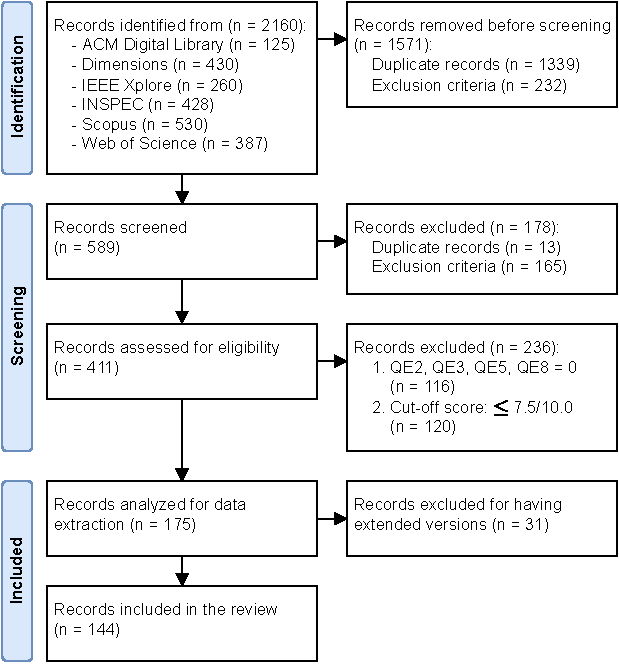
\includegraphics[width=\columnwidth]{figures/selection.pdf}
  \caption{PRISMA flow diagram for the selection process}
  \label{fig:methodology:prisma-flow}
\end{figure}

\subsubsection{Identification}

In the identification phase of this review, the search strategy is applied to all databases. \citetitle{methodology:search:db:acm}, \citetitle{methodology:search:db:dimensions}, \citetitle{methodology:search:db:inspec}, \citetitle{methodology:search:db:scopus}, and \citetitle{methodology:search:db:wos} data sources only require a single inquiry to obtain the search results. Given the limitation of the \citetitle{methodology:search:db:ieee-xplore} in terms of the number of wildcards mentioned in Section~\ref{sec:methodology:search}, the number of records for this source presented in Figure~\ref{fig:methodology:prisma-flow} represents the results of 7 inquiries (using the fields title, abstract, author keywords, IEEE terms, INSPEC controlled terms, and the INSPEC uncontrolled ones, respectively) after removing the duplicates with the support of \citetitle{methodology:parsifal}. Although the total number of search results found is 2160, \citetitle{methodology:parsifal} is used to remove duplicates from different data sources, excluding 1339 records. Following the duplicates removal, the exclusion criteria defined in Section~\ref{sec:methodology:search} exclude 232 works from the review. This exclusion is possible due to \citetitle{methodology:search:db:inspec}, \citetitle{methodology:search:db:scopus}, or \citetitle{methodology:search:db:wos} having filters related to the publication's type, subject area, and language.

The works excluded from the search results also include the ones that do not meet the exclusion criteria E4 and E7. For the first one, a Python script available in the GitHub repository of this review searches studies with a number of pages lower or equal to 4. Even though short papers have a maximum number of 3 pages, the papers with 4 pages do not usually present a detailed methodology.
As for the E7 exclusion criterion, some works are possible to remove from the review by searching in their title for the term ``dataset''.
All excluded articles of this review are double-checked to certify if the exclusion criteria are correctly applied. For example, articles published in the Remote Sensing journal from MDPI do not meet the E3 criterion. Indeed, the Journal Citations Reports from Clarivate classifies it by the following categories: Remote Sensing, Geosciences Multidisciplinary, Environmental Sciences, and Imaging Science \& Photographic Technology. However, most search results from this journal found in the identification phase are directly related to the topic of this review and the respective subject areas. Thus, in these cases and in other ones related to the remaining exclusion criteria, the decision is reverted to consider the initially rejected studies for the next phase of the review.

\subsubsection{Screening}

Next, the screening phase in this review consists of reading the title and abstract of the publications and rejecting the ones that meet the exclusion criteria. However, the initially rejected papers have another assessment for validating the exclusion. The analysis of the results and conclusions of these publications considering the exclusion criteria either confirms the exclusion decision or reverses it to eligible works for quality assessment. As a result of the screening phase, 178 studies are rejected from the initial identified 589 works. The duplicate records found in screening and removed manually are due to titles with invalid characters originated by exporting the search results from the \citetitle{methodology:search:db:dimensions}~database.

\subsubsection{Quality assessment}

The quality evaluation in this review of the selected works from screening follows the 8 Quality Evaluation (QE) criteria presented in Table~\ref{tab:methodology:quality-assessment}. All of them are subjective metrics derived from the authors' analysis of the eligible works. The score column establishes the possible values for these metrics, in which the minimum, intermediate, and maximum values correspond to none, partial, and full compliance, respectively.
Furthermore, QE1, QE2, QE4, and QE8 are subjective metrics that focus on the details provided in the papers, specifically, if the discussion of the related work, the proposed methodology, the experimental setup, and the results are detailed and thoroughly analyzed in the publication, respectively.
The possible scores for QE3 are twice the value of QE1, QE2, QE4, and QE8 due to this metric being directly related to the topic of the review. A work focusing on both localization and mapping problems will have a score of 2.0 (full compliance). If the study only focuses on one of these problems or none of them, the scores will be 1.0 or 0.0, i.e., partial or no compliance, respectively.
QE5 evaluates the long-term results of the eligible studies and is either 2.0 (full) or 0.0 (no compliance). This metric has the same range as QE3 for similar reasons, given the focus of this review on long-term localization and mapping algorithms.
The definition of long-term experiments for assigning full compliance in QE5 is the following one: dynamic changing environments (e.g., dynamic elements or semi-static ones), increasing environment and/or feature maps in terms of their size, redundant data removal, and/or varying conditions (e.g., different seasons of the year or lighting conditions).
Also, QE6 and QE7 can only be 1.0 or 0.0. The former criterion intends to highlight works that compare themselves to the state of the art and/or ground-truth data. The latter emphasizes the importance of having available either the implementation of the proposed methodology or the data used in the experiments for other works to be able to compare the proposed methodologies.
Lastly, considering the possible scores for the QE criteria presented in Table~\ref{tab:methodology:quality-assessment}, each work can only have a  maximum score of 10.0.

\begin{table}[h]
  \renewcommand{\arraystretch}{1.25}
  \setlength{\tabcolsep}{3pt}
  \caption[Quality evaluation criteria and score range]{Quality evaluation criteria and score range}
  \vspace{0.5em}
  \label{tab:methodology:quality-assessment}
  \centering
  {\scriptsize
  \begin{tabular}{c m{0.68\columnwidth} c}

\hline
\textbf{QE\#} & \textbf{Criteria} & \textbf{Score}\\
\hline
QE1 &
Does the paper have an updated state of the art on long-term localization and mapping? &
\{0.0, 0.5, 1.0\}\\
\hline
QE2 &
Is the methodology appropriate and detailed? &
\{0.0, 0.5, 1.0\}\\
\hline
QE3 &
Does the methodology consider both localization and mapping problems? &
\{0.0, 1.0, 2.0\}\\
\hline
QE4 &
Is the hardware and/or software used in the experiments detailed? &
\{0.0, 0.5, 1.0\}\\
\hline
QE5 &
Does the paper presents any kind of long-term experimental results? &
\{0.0, 2.0\}\\
\hline
QE6 &
Does the paper presents comparative results with other methods and/or ground-truth data? &
\{0.0, 1.0\}\\
\hline
QE7 &
Does the work's implementation and/or the data used in the experiments are publicly available? &
\{0.0, 1.0\}\\
\hline
QE8 &
Is the discussion of the results and conclusions appropriate and detailed? &
\{0.0, 0.5, 1.0\}\\
\hline

  \end{tabular}}
\end{table}

After evaluating the 411 eligible works accordingly to the previously discussed QE criteria (the scores of each record are available in the GitHub repository), the first conclusion of the authors is that works with a non-detailed or not appropriate methodology, results' discussion, or conclusions should not be included in the review. Another conclusion is relative to rejecting works that do not consider either localization or mapping problems, or do not present any long-term experimental results, given the focus of this review on the long-term localization and mapping problem for mobile robots. Furthermore, the quality assessment phase should consider a cut-off score to filter works with low quality scores. Consequently, the assessment phase considers the following two reasons to reject a record:

\begin{enumerate}\setlength\itemsep{-0.5em}
\item QE2, QE3, QE5, QE8: reject works with a 0.0 (no compliance) score;
\item cut-off score: reject works with a score lower or equal to 7.5/10.0.
\end{enumerate}

The distribution of the evaluation scores and the QE criteria itself justify the selection of a 7.5/10.0 cut-off score. 
Figure~\ref{fig:methodology:qe} illustrates the scores distribution for all eligible works versus the scores of the ones that pass the first criterion defined previously for the QE phase (related to the compliance on the QE2, QE3, QE5, and QE8 criteria). The assessment of this criterion rejects 116 records (28\%) of the 411 eligible works (see Figure~\ref{fig:methodology:prisma-flow}). 
Even though the distribution of the evaluation scores changes significantly in the range of scores lower or equal to 7.5/10.0, as observed between Figures~\ref{fig:methodology:qe:qe_wo-r1} and~\ref{fig:methodology:qe:qe}, only one work with a score higher than 7.5 is rejected due to not having a detailed and appropriate discussion of the results. This result indicates that interesting works are associated with high scores, as intended when using a quality assessment methodology, while also suggests that the range between 8.0 and 10.0 have the most interesting and higher quality works that are compatible with the focus of this review on long-term localization and mapping. Although only assessing the eligible works would seem to lead to the same results in terms of records included in the review, the rejection criterion on QE2/3/5/8 prevents outliers related to the quality assessment.
From the remaining 295 eligible works, cut-off scores from 7.5 up to 8.5 have the following corresponding rejection rates:

\begin{itemize}\setlength\itemsep{-0.5em}
\item 7.5/10.0: 120 records (41\%) $\rightarrow$ include 175 records
\item 8.0/10.0: 160 records (54\%) $\rightarrow$ include 135 records
\item 8.5/10.0: 203 records (69\%) $\rightarrow$ include 92 records
\end{itemize}

\begin{figure}[h]
  \centering
  \subfloat[][]{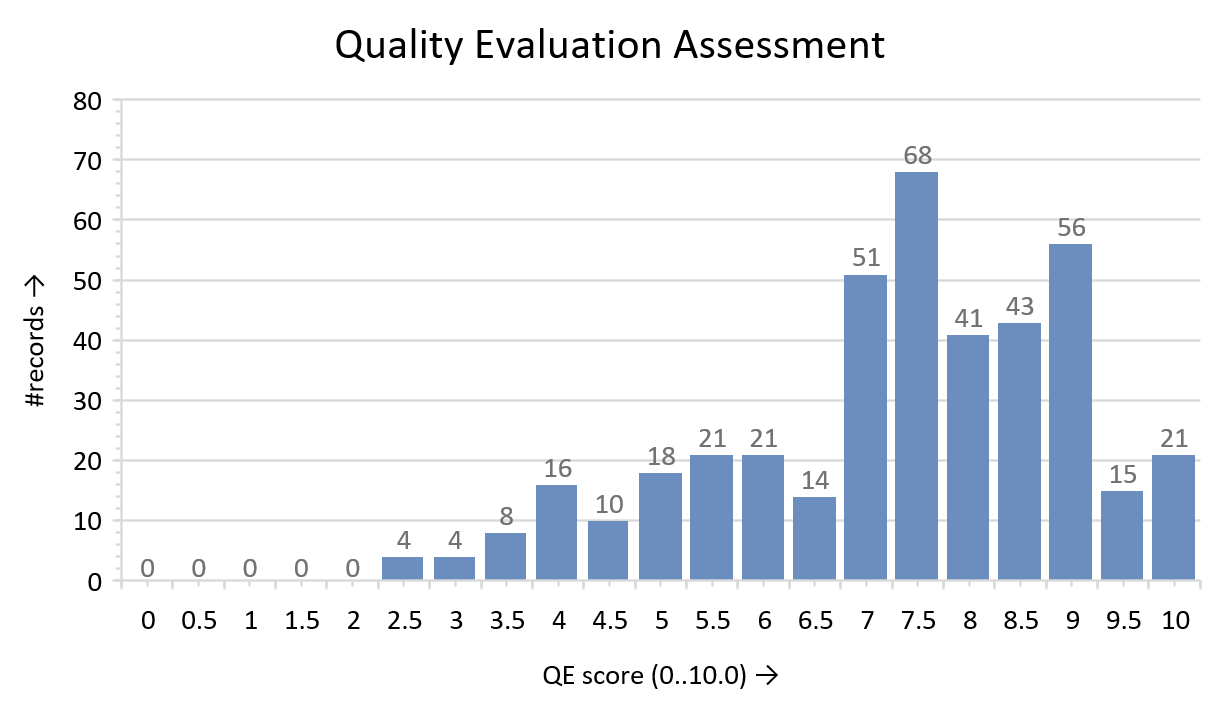
\includegraphics[width=\columnwidth]{figures/qe.png}%
  \label{fig:methodology:qe:qe}}
  \linebreak
  \subfloat[][]{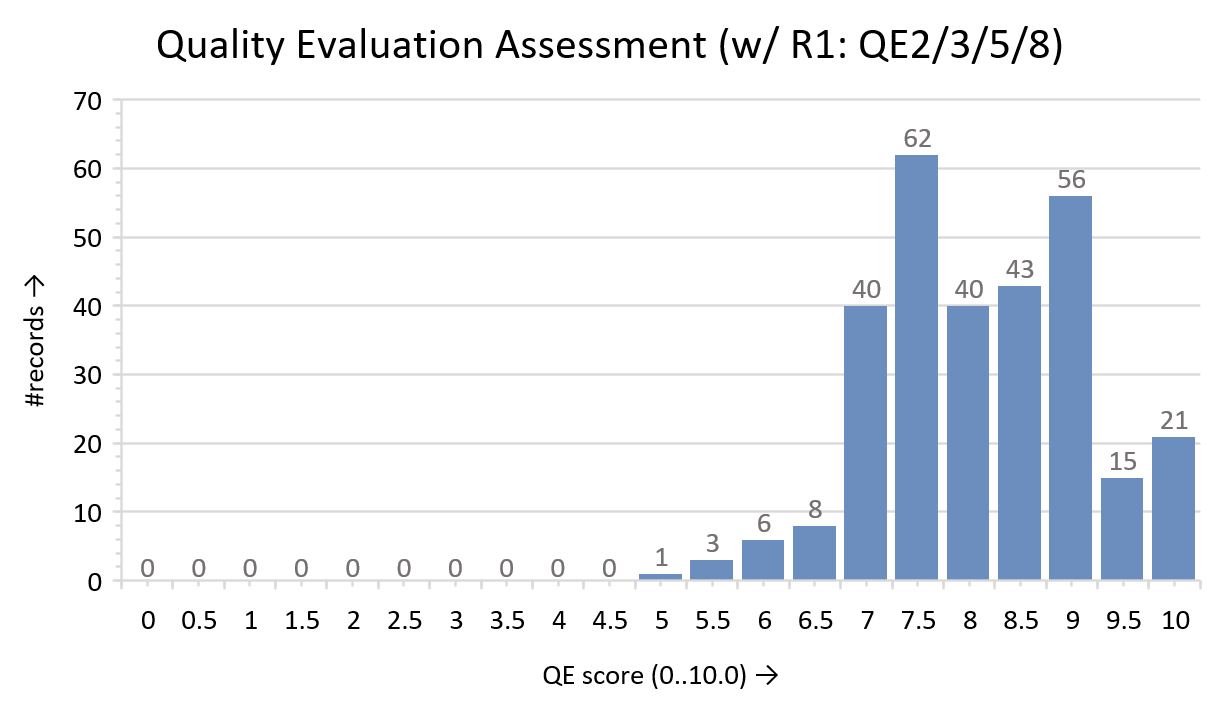
\includegraphics[width=\columnwidth]{figures/qe_wo-r1.png}%
  \label{fig:methodology:qe:qe_wo-r1}}
  \caption{Distribution of the quality evaluation scores obtained from assessing the eligible works considered in the review: (a) all eligible works; (b) works that pass the rejection criterion during the QE assessment related to QE2/3/5/8 = 0.0 (no compliance)}
  \label{fig:methodology:qe}
\end{figure}

The 8.5 cut-off score would not be suitable because methods that focus only on localization or not having either the implementation or the experimental data publicly available would be obligated to have maximum scores in the other criteria to be included in the review. In these cases, a work would have a maximum score of 9.0 due to partial compliance on QE3 or no compliance on the QE7 criteria. Likewise, a cut-off score of 8.0 would only leave a margin for having a single partial compliance on QE1, QE2, QE4 or QE8 criteria in similar cases, even though it would reject 160/295 (54\%) records. Therefore, the 7.5/10.0 cut-off score is more appropriate for the quality assessment phase in this review by leaving margin for works to have partial compliance in more than one criterion. Indeed, this cut-off score allows an article with no public data and/or implementation (e.g., due to confidentiality agreements) to have up to four criteria with partial compliance, depending on the criterion's maximum score or if the work has available the experiments data and/or implementation. Another example is articles that only focus on localization or mapping. In these cases, the work could have no public implementation, even though requiring a maximum score on all other criteria, or, if the work has public data or implementation available, two other criteria could have partial compliance.

Overall, as illustrated in Figure~\ref{fig:methodology:prisma-flow}, the quality assessment of the 411 eligible works considering the two rejection criteria previously mentioned leads to rejecting a total of 236 (57\%) records. As a result, the remaining 175 records will be analyzed for data extraction.

\subsection{Data extraction}
\label{sec:methodology:data}

The data extraction process analyzes the records selected after the quality assessment phase and extracts information from these works. In the scope of this review, the data items required for each record are the following ones:

\begin{itemize}\setlength\itemsep{-0.5em}
\item \textbf{DE1 -- Long-term considerations}: long-term factors the works consider in their approach and experiments;
\item \textbf{DE2 -- Localization method}: how the robot localizes itself and the type of localizer;
\item \textbf{DE3 -- Mapping method}: how the map is maintained and the type of the map;
\item \textbf{DE4 -- Multi-robot}: if the proposed methodologies consider multi-robot systems;
\item \textbf{DE5 -- Execution mode}: offline, online, or if requires both;
\item \textbf{DE6 -- Environment and domain}: type of environment and domain of the robot;
\item \textbf{DE7 -- Sensory setup}: which sensors are considered in the proposed methodologies and experiments;
\item \textbf{DE8 -- Evaluation metrics}: which metrics are used in the experiments to evaluate the performance;
\item \textbf{DE9 -- Ground-truth}: how the ground-truth data is obtained or its type, if available;
\item \textbf{DE10 -- Datasets}: if and which public datasets are used in the experiments;
\item \textbf{DE11 -- Maximum traveled distance}: if available, maximum traveled distance in continuous operation during the experiments;
\item \textbf{DE12 -- Maximum time interval}: if available, maximum time interval in continuous operation during the experiments.
\end{itemize}

Although the data extraction phase in a systematic literature review usually does not remove any records, 31 of the analyzed 179 works have extended versions of the proposed methodologies, more detailed ones, or equivalent methods applied in different conditions.
Therefore, these records are not included in the review to improve the discussion section in terms of singularity and originality of proposed approaches for the long-term localization and mapping problem.
Appendix~\ref{a1:rmv-records} presents the removed versions and their association with the records included in the review. The extracted information helped identifying the corresponding extended and more complete versions of these works.

Consequently, 144 original works are included in this review for an overview of these records in Section~\ref{sec:results}, and their synthesis and discussion in Section~\ref{sec:discussion}. The information relative to the 12 data items for each of the included records is available in Appendix~\ref{a2:data-extraction} and also in the public GitHub repository. The included works represent 35\% of the 411 eligible records for this review. This result indicates that the methodology followed in this review led to a high percentage of quality results.

\section{Results Overview}
\label{sec:results}

Section intends to overview the results overall, not focused at this point of synthesizing the results in different category analysis. First, the data sources in which the records are found following the methodology proposed in Section~\ref{sec:methodology} are analyzed to evaluation the impact each source had in obtaining the included records in the review. Next, the tool VOSviewer (\textcolor{red}{PUT HERE A  REFERENCE}) is used to obtain a keywords co-occurrence and co-authorship networks for analysis in the review. The former tries to find the keywords more found within the included records and tries to relate these to the discussion part of the review. The latter focus on find clusters of authors that work together, and possibly relate these clusters with research areas, nationalities, research centers, among other analysis items. Furthermore, the number of publications accordingly to their publication year of the included works is discussed to evaluate if there is any trend in time, and also when the subject area of long-term SLAM gain relevance. Finally, the publication venue analysis (either journal or conference) shows the top 10 journals and conferences in which the included works were published in, to try to find trends of publications.

\subsection{Data source}

The number of records identified by each data source following the methodology described in Section~\ref{sec:methodology} for only the included works considered for discussion are the following ones:

\begin{itemize}\setlength\itemsep{-0.5em}
\item \citetitle{methodology:search:db:acm}: 0 records (0.00\%);
\item \citetitle{methodology:search:db:dimensions}: 65 records (45.14\%);
\item \citetitle{methodology:search:db:ieee-xplore}: 67 records (46.53\%);
\item \citetitle{methodology:search:db:inspec}: 101 records (70.14\%);
\item \citetitle{methodology:search:db:scopus}: 122 records (84.72\%);
\item \citetitle{methodology:search:db:wos}: 104 records (72.22\%).
\end{itemize}

\textcolor{red}{DETECTED A BUG WHEN SEARCHING IN THE ACM DATABASE... NEED TO CORRECT URGENTLY!!! 5 RESULTS ARE NOW MAXIMUM 127 RESULTS...}
					
\begin{table}[h]
  \centering
  \caption{Identification percentage matrices of the 144 records included in the review for the possible pairwise correspondence of data sources: (a) only on both databases (intersection); (b) on either ones (union). Legend: dim -- \citetitle{methodology:search:db:dimensions}, ieee -- \citetitle{methodology:search:db:ieee-xplore}, inspec -- \citetitle{methodology:search:db:inspec}, scopus -- \citetitle{methodology:search:db:scopus}, wos -- \citetitle{methodology:search:db:wos}}
  \label{tab:results:source}
  \subfloat[][]{%
  \begin{tabular}{l|P{0.1\columnwidth}P{0.1\columnwidth}P{0.1\columnwidth}P{0.1\columnwidth}P{0.1\columnwidth}}
\textit{A} $\cap$ \textit{B} & \textbf{dim} & \textbf{ieee} & \textbf{inspec} & \textbf{scopus} & \textbf{wos}\\
\hline
\textbf{dim} & -- & 18.75\% & 31.25\% & 43.75\% & 43.06\%\\
\textbf{ieee} & -- & -- & 40.97\% & 42.36\% & 34.03\%\\
\textbf{inspec} & -- & -- & -- & 61.11\% & 48.61\%\\
\textbf{scopus} & -- & -- & -- & -- & 64.58\%\\
\textbf{wos} & -- & -- & -- & -- & --\\
\hline
  \end{tabular}\label{tab:results:source:intersect}%
  }
  \linebreak
  \subfloat[][]{%
  \begin{tabular}{l|P{0.1\columnwidth}P{0.1\columnwidth}P{0.1\columnwidth}P{0.1\columnwidth}P{0.1\columnwidth}}
\textit{A} $\cup$ \textit{B} & \textbf{dim} & \textbf{ieee} & \textbf{inspec} & \textbf{scopus} & \textbf{wos}\\
\hline
\textbf{dim} & -- & 72.92\% & 84.03\% & 86.11\% & 74.31\%\\
\textbf{ieee} & -- & -- & 75.69\% & 88.89\% & 84.72\%\\
\textbf{inspec} & -- & -- & -- & 93.75\% & 93.75\%\\
\textbf{scopus} & -- & -- & -- & -- & 92.36\%\\
\textbf{wos} & -- & -- & -- & -- & --\\
\hline
  \end{tabular}\label{tab:results:source:union}%
  }
\end{table}

\subsection{Keywords co-occurrence}

\begin{figure}[!t]
  \centering
  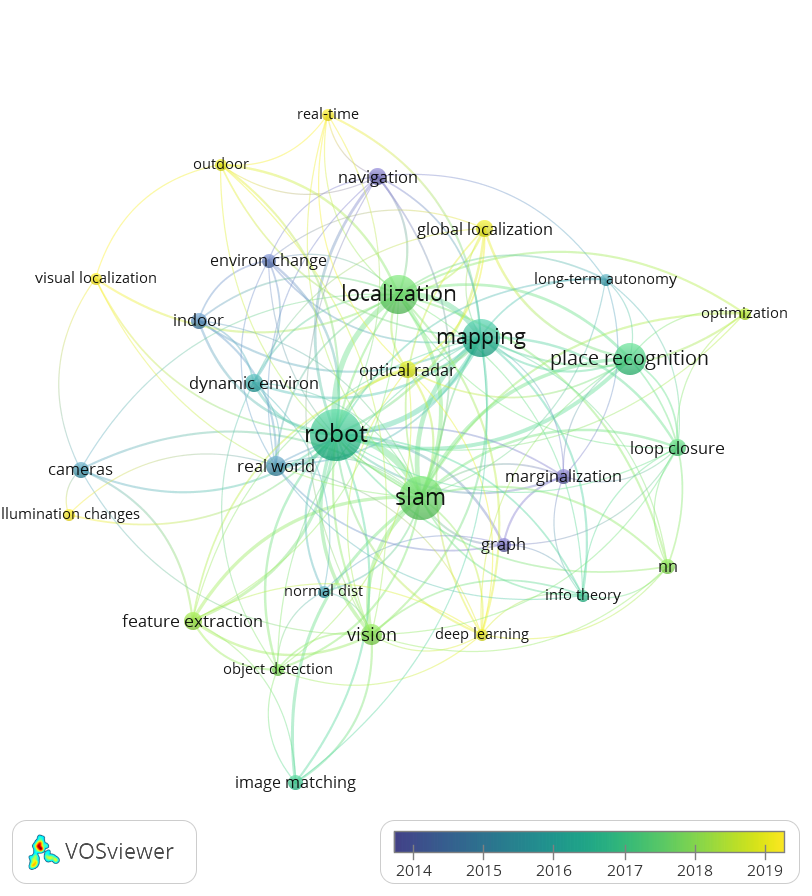
\includegraphics[width=\columnwidth]{figures/kw.png}
  \caption{Keywords co-occurrence analysis generated by VOSviewer}
  \label{fig:results:kw}
\end{figure}

\subsection{Co-authorship analysis}

\begin{figure}[!t]
  \centering
  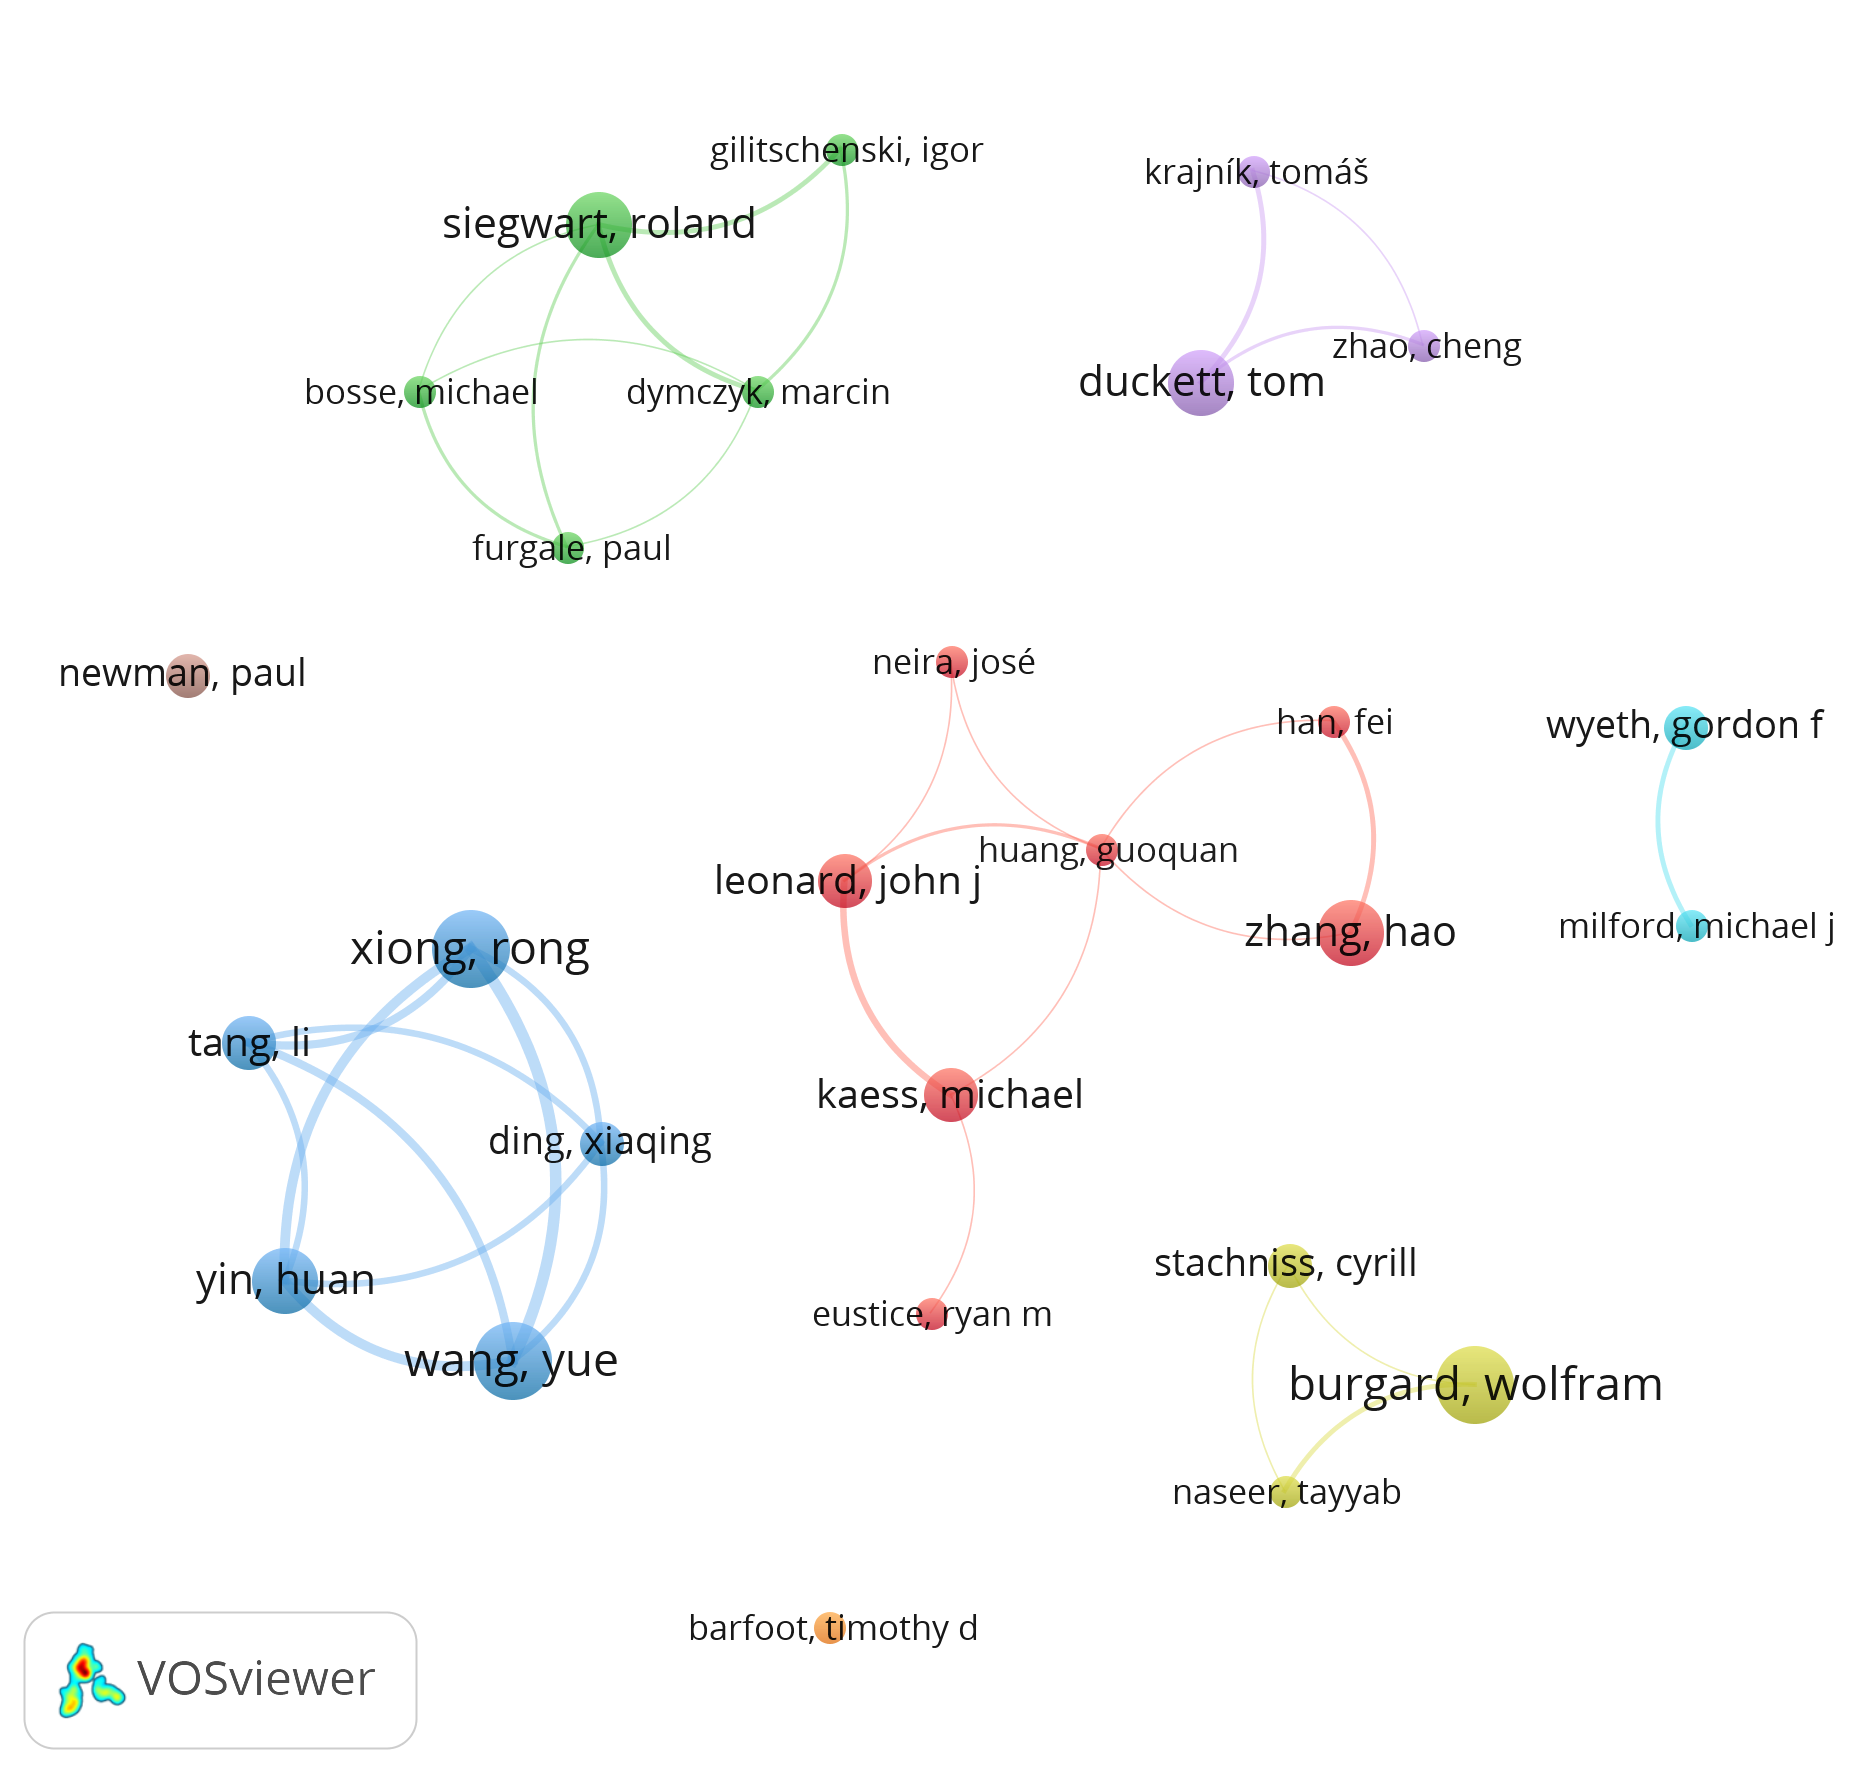
\includegraphics[width=\columnwidth]{figures/authors.png}
  \caption{Co-authorship analysis generated by VOSviewer}
  \label{fig:results:authors}
\end{figure}

\subsection{Year of publication}

\begin{figure}[!t]
  \centering
  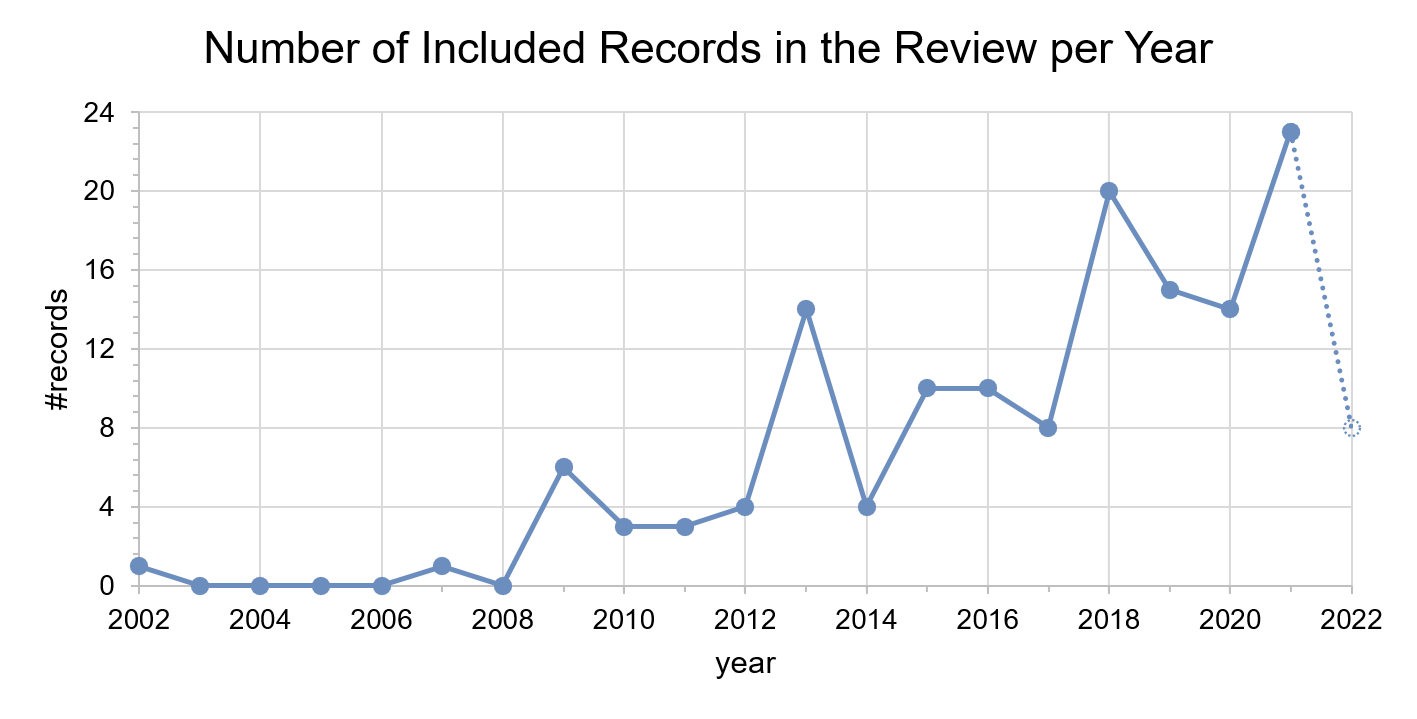
\includegraphics[width=\columnwidth]{figures/year.png}
  \caption{Number of included publications in the review per year}
  \label{fig:results:year}
\end{figure}

\subsection{Publication venue}

\section{Discussion}
\label{sec:discussion}

\subsection{Invariant features}

trabalhos / abordagens que se foca em formulação de features invariantes a condições externas e que sejam estáveis a long-term

\subsection{Place recognition}

trabalhos / abordagens para reconhecimento de espaços já guardados no mapa atual ou por via de experience-based techniques, sequências de imagens, vocabulários, etc.

\subsection{Environment dynamics}

trabalhos / abordagens para modelação e / ou rejeição da dinâmica do ambiente (mapa, features, etc.)

\subsection{Redundancy data rejection}

trabalhos / abordagens que se foquem em mecanismos de rejeição de dados redundantes no mapa (que também influencia tanto memória como tempo de processamento)

\subsection{Memory management}

trabalhos / abordagens que se focam em mecanismos de gestão de memória que sejam independentes da qualidade ou redundância do mapa

\subsection{Multiple sessions}

trabalhos / abordagens que se foquem na questão de multi-session

talvez incluir global localization / relocalization? Or it is already included in this section?

\subsection{Datasets}

Characteristics of datasets used in the results' articles section.

Possibly add other datasets not mentioned in the works selected for the article.

Comparative table or summary of the characteristics (types of sensors, ground-truth, timeframe - month, week, day, consideration or not of dynamic environments and/or varying conditions).

\subsection{Performance measures}

types of performance measures used to evaluate algorithms focusing on long-term perspective

\section{Challenges and Future Directions}
\label{sec:challenges:future}

\section{Limitations of the Study}
\label{sec:limitations}

Section to discuss possible limitations of the study (timeframe, wider approach, etc.).

\begin{itemize}\setlength\itemsep{-0.5em}
\item only one query for discussion: e.g., for searching datasets, possibly, a different query should have been used
\item overview long-term SLAM vs in-depth analysis and discussion of each type of techniques: our review synthesizes all types of techniques, if the reader wants an in-depth analysis, different reviews should be performed
\item limited information on the experiments conditions (traveled distance, duration, etc.) given by the authors
\end{itemize}

\section{Conclusions}
\label{sec:conclusions}

ssss



\section*{Acknowledgments}

This study was supported by FCT -- Fundação para a Ciência e a Tecnologia and INESC TEC -- Institute for Systems and Computer Engineering, Technology and Science.

\section*{ORCID}

\noindent \textit{Ricardo B. Sousa} 
\includegraphics[width=1em]{orcid.pdf} \href{https://orcid.org/0000-0003-4537-5095}{https://orcid.org/0000-0003-4537-5095}

\noindent \textit{H\'{e}ber M. Sobreira} 
\includegraphics[width=1em]{orcid.pdf} \href{https://orcid.org/0000-0002-8055-1093}{https://orcid.org/0000-0002-8055-1093}

\noindent \textit{Ant\'{o}nio Paulo Moreira} 
\includegraphics[width=1em]{orcid.pdf} \href{https://orcid.org/0000-0001-8573-3147}{https://orcid.org/0000-0001-8573-3147}



%% BIBLIOGRAPHIC REFERENCES

\printbibliography

%\bibliographystyle{unsrt}
%\bibliography{references.bib}



%% AUTHORS BIOGRAPHIES

\newpage

\noindent \textbf{Ricardo B. Sousa} obtained a Master of Science (M.Sc.) degree in Electric and Computers Engineering (ECE) at Faculty of Engineering of the University of Porto (FEUP), in 2020.
He is currently working towards the Ph.D. degree in electrical and computer engineering with FEUP, and he has a graduate research scholarship from FCT -- Fundação para a Ciência e a Tecnologia at the Centre for Robotics in Industry and Intelligent Systems from INESC TEC.
Also, he is an invited assistant lecturing the courses Software Design and Industrial Informatics from the M.Sc. in ECE at FEUP.
His research interests include robotics, sensor fusion, and localization and mapping for autonomous robots.

\vspace{1em}

\noindent \textbf{H\'{e}ber M. Sobreira} was born in Leiria, Portugal, in July 1985. He graduated with an M.Sc. degree (2009) and a Ph.D. degree (2017) in Electrical Engineering from the University of Porto. Since 2009, he has been developing his research within the Centre for Robotics in Industry and Intelligent Systems at INESC TEC. His main research areas are navigation and control of indoor autonomous vehicles.

\vspace{1em}

\noindent \textbf{Ant\'{o}nio Paulo Moreira} graduated with a degree in electrical engineering at the University of Oporto, in 1986. Then, he pursued graduate studies at University of Porto, obtaining a M.Sc. degree in electrical engineering -- systems in 1991 and a Ph.D. degree in electrical engineering in 1998. Presently, he is Associate Professor with tenure at the Faculty of Engineering of the University of Porto and researcher and head of the Centre for Robotics in Industry and Intelligent Systems at INESC TEC. His main research interests are process control and robotics.



%% APPENDIXES

\cleardoublepage

\appendix

\onecolumn

\section{Records Removed at the Data Extraction Phase}
\label{a1:rmv-records}

\begin{table*}[!h]
  \renewcommand{\arraystretch}{1.25}
  \setlength{\tabcolsep}{3pt}
  \caption[Records not included in the review for having extended, more detailed or similar versions]{Records not included in the review for having extended, more detailed or similar versions}
  \vspace{0.5em}
  \label{tab:a1:rmv-records}
  \centering
  {\scriptsize
  \begin{tabular}{l l}

\hline
\textbf{Included} & \textbf{Corresponding versions removed from the review}\\
\hline
\cite{hochdorfer-et-al:2009:5339626}, \cite{hochdorfer-schlegel:2009} &
\cite{hochdorfer-schlegel:2009:5354433}, \cite{hochdorfer-schlegel:2010:5651229}\\
\cite{dayoub-et-al:2011:013} &
\cite{dayoub-duckett:2008:4650701}\\
\cite{latif-et-al:2012:6385879} &
\cite{latif-et-al:2013:030}, \cite{latif-et-al:2013:0278364913498910}\\
\cite{bacca-et-al:2013:003} &
\cite{bacca-et-al:2010:291}, \cite{bacca-et-al:2011:008}\\
\cite{kawewong-et-al:2013:826410} & 
\cite{kawewong-et-al:2010:2587}, \cite{kawewong-et-al:2011:0278364910371855}, \cite{kawewong-et-al:2011:007}\\
\cite{paul-newman:2013:0278364913509859} &
\cite{paul-newman:2011:5980404}\\
\cite{carlevaris-bianco-et-al:2014:2347571} &
\cite{carlevaris-bianco-eustice:2013:6696478}\\
\cite{neubert-et-al:2015:005} &
\cite{neubert-et-al:2013:6698842}\\
\cite{ozog-et-al:2016:21582} &
\cite{ozog-eustice:2014:6907415}\\
\cite{biswas-veloso:2017:005} &
\cite{biswas-veloso:2014:6907435}\\
\cite{griffith-pradalier:2017:21664} &
\cite{griffith-pradalier:2016:1}\\
\cite{krajník-et-al:2017:2665664} &
\cite{krajník-et-al:2016:7759671}\\
\cite{arroyo-et-al:2018:7} &
\cite{arroyo-et-al:2015:7140088}, \cite{arroyo-et-al:2016:7795672}\\
\cite{han-et-al:2018:3} &
\cite{zhang-et-al:2016:043}\\
\cite{han-et-al:2018:2856274} &
\cite{han-et-al:2018}\\
\cite{mactavish-et-al:2018:21838} &
\cite{paton-et-al:2016:7759303}\\
\cite{bürki-et-al:2019:21870} &
\cite{bürki-et-al:2016:7759609}, \cite{bürki-et-al:2018:8500432}\\
\cite{labbé-michaud:2019:21831} &
\cite{labbé-michaud:2011:6048225}, \cite{labbé-michaud:2013:2242375}, \cite{labbé-michaud:2018:5}\\
\cite{gao-zhang:2020:9196906} &
\cite{gao-zhang:2020:6604}\\
\cite{berrio-et-al:2021:3094485} &
\cite{berrio-et-al:2019:8814189}\\
\cite{piasco-et-al:2021:6} &
\cite{piasco-et-al:2019:8794221}\\
\cite{bouaziz-et-al:2022:4} &
\cite{bouaziz-et-al:2021:9378614}\\
\hline

  \end{tabular}}
\end{table*}


\clearpage
\begin{landscape}
\clearpage

\section{Data Extraction Results of the Included Records in the Systematic Literature Review on Long-Term Localization and Mapping for Mobile Robots}
\label{a2:data-extraction}

\begin{tiny}

\begin{longtable}{p{0.08\textwidth}p{0.08\textwidth}p{0.08\textwidth}p{0.08\textwidth}p{0.08\textwidth}p{0.08\textwidth}p{0.08\textwidth}p{0.08\textwidth}p{0.08\textwidth}p{0.08\textwidth}p{0.08\textwidth}p{0.08\textwidth}p{0.08\textwidth}}
  %\renewcommand{\arraystretch}{1.25}
  %\setlength{\tabcolsep}{3pt}
  %{\scriptsize
  \caption{Data extraction items retrieved from the included records in the review}
  \vspace{0.5em}
  \label{tab:a2:data-extraction}\\

%% FIRST TABLE HEADER
\hline
\textbf{Ref.} & \textbf{DE1} & \textbf{DE2} & \textbf{DE3} & \textbf{DE4} & \textbf{DE5} & \textbf{DE6} & \textbf{DE7} & \textbf{DE8} & \textbf{DE9} & \textbf{DE10} & \textbf{DE11} & \textbf{DE12}\\
\hline
\endfirsthead

%% TABLE HEADER IN THE FOLLOWING PAGES
\multicolumn{13}{l}{\itshape{\tablename\ \thetable{}: continued from previous page}}
\vspace{0.5em}\\
\hline
\textbf{Ref.} & \textbf{DE1} & \textbf{DE2} & \textbf{DE3} & \textbf{DE4} & \textbf{DE5} & \textbf{DE6} & \textbf{DE7} & \textbf{DE8} & \textbf{DE9} & \textbf{DE10} & \textbf{DE11} & \textbf{DE12}\\
\hline
\endhead

%% TABLE FOOTER
\hline
\endfoot
\hline
\endlastfoot



%% TABLE CONTENT
\cite{davison-murray:2002:1017615} \\
\hline
\cite{filliat:2007:364080} \\
\hline
\cite{konolige-bowman:2009:5354121} \\
\hline
\cite{bosse-zlot:2009:009} \\
\hline
\cite{biber-duckett:2009:0278364908096286} \\
\hline
\cite{hochdorfer-schlegel:2009} \\
\hline
\cite{hochdorfer-et-al:2009:5339626} \\
\hline
\cite{nuske-et-al:2009:20306} \\
\hline
\cite{glover-et-al:2010:5509547} \\
\hline
\cite{kretzschmar-et-al:2010:2} \\
\hline
\cite{ikeda-tanaka:2010:5509579} \\
\hline
\cite{dayoub-et-al:2011:013} \\
\hline
\cite{kretzschmar-et-al:2011:6048060} \\
\hline
\cite{pirker-et-al:2011:6048253} \\
\hline
\cite{walcott-bryant-et-al:2012:6385561} \\
\hline
\cite{kretzschmar-stachniss:2012:0278364912455072} \\
\hline
\cite{maddern-et-al:2012:6224622} \\
\hline
\cite{latif-et-al:2012:6385879} \\
\hline
\cite{kawewong-et-al:2013:826410} \\
\hline
\cite{bacca-et-al:2013:003} \\
\hline
\cite{ball-et-al:2013:9} \\
\hline
\cite{einhorn-gross:2013:6698849} \\
\hline
\cite{tipaldi-et-al:2013:0278364913502830} \\
\hline
\cite{huang-et-al:2013:6698835} \\
\hline
\cite{johannsson-et-al:2013:6630556} \\
\hline
\cite{oberländer-et-al:2013:6766479} \\
\hline
\cite{saarinen-et-al:2013:0278364913499415} \\
\hline
\cite{biswas-veloso:2013:0278364913503892} \\
\hline
\cite{paul-newman:2013:0278364913509859} \\
\hline
\cite{nguyen-et-al:2013:004} \\
\hline
\cite{maddern-et-al:2013:036} \\
\hline
\cite{churchill-newman:2013:0278364913499193} \\
\hline
\cite{pomerleau-et-al:2014:6907397} \\
\hline
\cite{murphy-sibley:2014:6907022} \\
\hline
\cite{carlevaris-bianco-et-al:2014:2347571} \\
\hline
\cite{williams-et-al:2014:0278364914531056} \\
\hline
\cite{einhorn-gross:2015:008} \\
\hline
\cite{pérez-et-al:2015:y} \\
\hline
\cite{li-et-al:2015:7139706} \\
\hline
\cite{mohan-et-al:2015:7139966} \\
\hline
\cite{dymczyk-et-al:2015:7139575} \\
\hline
\cite{rapp-et-al:2015:77} \\
\hline
\cite{vysotska-et-al:2015:7139576} \\
\hline
\cite{neubert-et-al:2015:005} \\
\hline
\cite{mur-artal-et-al:2015:2463671} \\
\hline
\cite{naseer-et-al:2015:7324181} \\
\hline
\cite{karaoguz-bozma:2016:4} \\
\hline
\cite{santos-et-al:2016:2516594} \\
\hline
\cite{dymczyk-et-al:2016:66} \\
\hline
\cite{dymczyk-et-al:2016:7759673} \\
\hline
\cite{gadd-newman:2016:7759843} \\
\hline
\cite{mazuran-et-al:2016:0278364915581629} \\
\hline
\cite{ozog-et-al:2016:21582} \\
\hline
\cite{mühlfellner-et-al:2016:21595} \\
\hline
\cite{an-et-al:2016:0} \\
\hline
\cite{taisho-kanji:2016:7866383} \\
\hline
\cite{han-et-al:2017:2662061} \\
\hline
\cite{biswas-veloso:2017:005} \\
\hline
\cite{griffith-pradalier:2017:21664} \\
\hline
\cite{naseer-et-al:2017:7989305} \\
\hline
\cite{krajník-et-al:2017:2665664} \\
\hline
\cite{ila-et-al:2017:0278364917691110} \\
\hline
\cite{latif-et-al:2017:016} \\
\hline
\cite{xin-et-al:2017:8310121} \\
\hline
\cite{bescos-et-al:2018:2860039} \\
\hline
\cite{opdenbosch-et-al:2018:00114} \\
\hline
\cite{han-et-al:2018:3} \\
\hline
\cite{han-et-al:2018:2856274} \\
\hline
\cite{cao-et-al:2018:2815956} \\
\hline
\cite{nobre-et-al:2018:8461111} \\
\hline
\cite{zhang-et-al:2018:1729881418780178} \\
\hline
\cite{zhu-et-al:2018:8500686} \\
\hline
\cite{mactavish-et-al:2018:21838} \\
\hline
\cite{sun-et-al:2018:2856268} \\
\hline
\cite{lázaro-et-al:2018:8594310} \\
\hline
\cite{zhang-et-al:2018:8460674} \\
\hline
\cite{chebrolu-et-al:2018:2849603} \\
\hline
\cite{yin-et-al:2018:8593562} \\
\hline
\cite{egger-et-al:2018:8593854} \\
\hline
\cite{arroyo-et-al:2018:7} \\
\hline
\cite{ouerghi-et-al:2018:s18040939} \\
\hline
\cite{siva-zhang:2018:8461042} \\
\hline
\cite{luthardt-et-al:2018:8569323} \\
\hline
\cite{chen-et-al:2018:2859916} \\
\hline
\cite{yu-et-al:2019:8961714} \\
\hline
\cite{boniardi-et-al:2019:003} \\
\hline
\cite{kim-et-al:2019:2897340} \\
\hline
\cite{berrio-et-al:2019:8814289} \\
\hline
\cite{wang-et-al:2019:8793499} \\
\hline
\cite{wu-wu:2019:8968599} \\
\hline
\cite{tang-et-al:2019:7} \\
\hline
\cite{bürki-et-al:2019:21870} \\
\hline
\cite{labbé-michaud:2019:21831} \\
\hline
\cite{zhang-et-al:2019:8814347} \\
\hline
\cite{schmuck-chli:2019:00071} \\
\hline
\cite{ganti-waslander:2019:00024} \\
\hline
\cite{ding-et-al:2019:8968550} \\
\hline
\cite{song-et-al:2019:8967749} \\
\hline
\cite{pan-et-al:2019:s19194252} \\
\hline
\cite{ali-et-al:2020:3389033} \\
\hline
\cite{qin-et-al:2020:103561} \\
\hline
\cite{martini-et-al:2020:s20216002} \\
\hline
\cite{karaoguz-bozma:2020:2} \\
\hline
\cite{yin-et-al:2020:2905046} \\
\hline
\cite{clement-et-al:2020:2967659} \\
\hline
\cite{wang-et-al:2020:9468884} \\
\hline
\cite{camara-et-al:2020:9196967} \\
\hline
\cite{gao-zhang:2020:9196906} \\
\hline
\cite{yang-et-al:2020:s20082432} \\
\hline
\cite{siva-et-al:2020:9340992} \\
\hline
\cite{qin-et-al:2020:9340939} \\
\hline
\cite{ding-et-al:2020:2942760} \\
\hline
\cite{yue-et-al:2020:9197072} \\
\hline
\cite{schaefer-et-al:2021:103709} \\
\hline
\cite{liu-et-al:2021:9561126} \\
\hline
\cite{kim-et-al:2021:3047421} \\
\hline
\cite{derner-et-al:2021:103676} \\
\hline
\cite{cao-et-al:2021:2962416} \\
\hline
\cite{singh-et-al:2021:9564866} \\
\hline
\cite{kurz-et-al:2021:9636530} \\
\hline
\cite{yin-et-al:2021:661199} \\
\hline
\cite{thomas-et-al:2021:9561701} \\
\hline
\cite{berrio-et-al:2021:3094485} \\
\hline
\cite{oh-eoh:2021:app11198976} \\
\hline
\cite{tsintotas-et-al:2021:103782} \\
\hline
\cite{sun-et-al:2021:9635886} \\
\hline
\cite{tang-et-al:2021:17298814211037497} \\
\hline
\cite{piasco-et-al:2021:6} \\
\hline
\cite{yin-et-al:2021:3061375} \\
\hline
\cite{meng-et-al:2021:3062647} \\
\hline
\cite{zhu-et-al:2021:9561584} \\
\hline
\cite{zeng-si:2021:6} \\
\hline
\cite{ali-et-al:2021:3100882} \\
\hline
\cite{xu-et-al:2021:3060741} \\
\hline
\cite{yang-et-al:2021:12054} \\
\hline
\cite{wang-et-al:2021:9739599} \\
\hline
\cite{hu-et-al:2022:1003907} \\
\hline
\cite{coulin-et-al:2022:3136241} \\
\hline
\cite{zhang-et-al:2022:3086822} \\
\hline
\cite{nguyen-et-al:2022:3094157} \\
\hline
\cite{bouaziz-et-al:2022:4} \\
\hline
\cite{du-et-al:2022:3028218} \\
\hline
\cite{xing-et-al:2022:22062} \\
\hline
\cite{hong-et-al:2022:02783649221080483} \\

\end{longtable}

\end{tiny}
\end{landscape}


\end{document}
